Проблема Борсука: $\Omega \subset \R^n, diam \Omega = sup_{x, y \in \Omega} |x - y| < \infty$.

Borsuk, 1933: $\Omega = \Omega_1 \sqcup \Omega_2 \sqcup \dots \sqcup \Omega_f$, $diam \Omega_i < diam \Omega$, $f(\Omega) = $ min число частей, на которое можно разбить $\Omega$; $f(n) = max_{\Omega} f(\Omega)$.

б.о.о. можно считать, что $diam \Omega = 1$, $\Omega$ можно считать замкнутым, выпуклым.

\Th $f(n) \geqslant (c + o(1))^{\sqrt{n}}, c \approx 1.203$

\Proof
p - простое; $n = 4p$; $V = \{\overline{x} = (x_1, \dots, x_n) : x_i \in \{+1, -1\}, x_1 = 1, x_2 \cdot \dots \cdot x_n = 1\}$

$|V| = 2^{n-2}$

\Lemma 1: $\forall x, y \in V: (x, y) \equiv 0 (4)$

\Lemma 2: $\forall x, y \in V: (x, y) \equiv 0 (p)$, p нечёт. Но тогда верно $\forall x, y \in V (x, y) = 0 || x = y$.

\Lemma 3: Пусть $W \subset V$: $\forall x, y \in W (x, y) \neq 0$. Тогда $|W| \leqslant \sum_{k=0}^{p-1}C_n^k$

Докажем лемму 3. Пусть $W = \{x_1, \dots, x_t\}$, $(x_i, x_j) \neq 0 \Leftrightarrow (x_i, x_j) \notequiv 0 (p)$. Тогда $x_i \to P_{x_i} \in \Z_p[y_1, \dots, y_n]: P_{x_i}(y) = \prod_{j=1}^{p=1} (j - (x_i, y))$. Модифицируем моном (редуцируем степени): удаляем все чётные степени, а вместо нечётных оставляем 1. Ура.

Используя лемму, построим контрпримеры и получим нижнюю оценку. Модифицируем $V$: $V \to V^* \subset \R^{n^2}$: $x = (x_1, \dots, x_n) \in V \to x^* = (x_1^2, x_1x_2, \dots, x_n^2) \in V^*$; соответствие взаимно однозначное, т.к. $x_1 = 1$, так как отрезок из первых $n$ элементов равен исходному вектору.

В силу того, что некоторые координаты у $x^*$ всегда равны 1 или то, что $x_ix_j = x_jx_i$ мы можем снизить размерность до $\R^{C_n^2}$

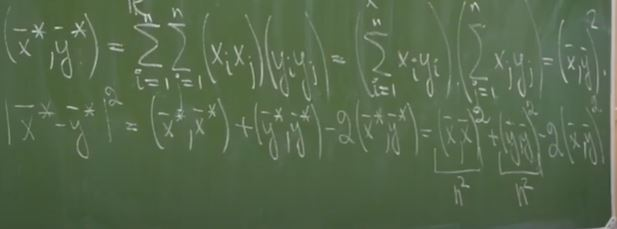
\includegraphics[]{images/73.JPG}

Таким образом, чтобы получить диаметр в $V^*$ нам нужно, чтобы $(x, y) = 0$.

$V = V_1^* \sqcup V_2^* \sqcup \dots \sqcup V_f^*$. Предположим, что $f < \frac{2^{n-2}}{\sum_{k=0}^{p-1} C_n^k}$; $V = V_1 \sqcup V_2 \sqcup \dots \sqcup V_f$ $\Rightarrow$ $\exists i : |V_i| \geqslant \frac{|V|}{f}$ (принцип Дирихле) $ > \sum_{k=0}^{p-1} C_n^k$ $\Rightarrow \exists x, y \in V_i: (x, y) = 0$ (лемма 3) $ \Rightarrow $ соответствующие $x^*, y^*$ реализуют диаметр $V^*$. Тогда $f(V^*) \geqslant \frac{2^{n-2}}{\sum_{k=0}^{p-1} C_n^k}$ $\Rightarrow$ $f(C_n^2) \geqslant \frac{2^{n-2}}{\sum_{k=0}^{p-1} C_n^k}$; $C_n^2 = d, d \sim \frac{n^2}{2} \Rightarrow n \sim \sqrt{2d}$

$\sum_{k=0}^{p-1} C_n^k = (\frac{1}{(1/4)^{1/4}(3/4)^{3/4}} + o(1))^n$, тогда $\frac{2^{n-2}}{\sum_{k=0}^{p-1} C_n^k} = (1.139 + o(1))^n = (1.139^{\sqrt{2}} + o(1))^{\sqrt{d}} = (1.203 + o(1))^{\sqrt{d}}$
\EndProof